\section{Scan Agent Installation and Configuration}\label{sec:scan-agent}

\subsection{Overview}

The Scan Agent is a service intended to run in a build environment that
matches the build environment generally used for the code.  The service executes
the \scaresolver and/or pre-scan scripting when events are handled by \cxoneflow that would invoke a scan.
The \scaresolver is typically executed in the code's build pipeline as a pre-step
for a multi-engine \cxone scan that includes an SCA scan.

The keys to a successful \scaresolver scan are generally:

\begin{itemize}
  \item The build tools used to obtain the dependency tree are the same versions and
    configurations as those used to build the code.
  \item The execution happens behind the enterprise firewall to allow for transitive
    dependency resolution of packages that are hosted in a private package repository.
\end{itemize}


\subsection{Installation and Configuration Pre-Requisites}

To install an instance of the Scan Agent, the following is required:

\begin{itemize}
  \item The Scan Agent installer appropriate for your target platform.
  \item An external message queue used by \cxoneflow and the Scan Agent (see Section \ref{sec:external-mq} for more details).
  \item A set of message queue credentials used by the Scan Agent (see Section \ref{sec:agent-mq-auth-req} for more details).
  \item A public key that is matched with a private key configured for use by the \cxoneflow server (see Section \ref{ref:server-key-pair} for more details).
  \item \scaresolver must be installed if intending to execute \scaresolver without a container.
  \item If intending to execute \scaresolver in a container:
  \begin{itemize}
    \item The system must have docker installed.
    \item The \toolkit build environment must be installed.
  \end{itemize}
\end{itemize}


\subsubsection{Message Queue Authorization}\label{sec:agent-mq-auth-req}

Scan Agents communicate with \cxoneflow using an AMQP message queue. Each Scan Agent 
must have a set of message queue credentials that limit how it can interact
with the message queue as appropriate for the agent's configured tags.

Table \ref{tab:agent-mq-user-perms} shows the permissions needed for the Scan Agent
to interact with the message queues.  Using a regular expression of "\texttt{\^{}cx:res:.*}" will allow
the agent to respond to events for any tag.  It is possible to limit which tags an agent can consume
by adding regular expressions that specify one or more tags at the end of the queue name.  For example, the
regular expression "\texttt{\^{}cx:res:.*(general|java-gradle)\$}" will limit the Scan Agent
to handling only tags \texttt{general} and \texttt{java-gradle}.

\begin{table}[ht]
  \caption{RabbitMQ User Permissions for the Scan Agents}
  \label{tab:agent-mq-user-perms}      
  \begin{tabularx}{\textwidth}{lcl}
      \toprule
      \textbf{Permission} & \textbf{Regular Expression} \\
      \midrule
      \texttt{Configure} & blank \\
      \midrule
      \texttt{Write} & \texttt{\^{}cx:res:.*} \\
      \midrule
      \texttt{Read} & \texttt{\^{}cx:res:.*} \\
      \midrule
      \bottomrule
  \end{tabularx}
\end{table}

Table \ref{tab:agent-mq-topic-perms} shows the topic permissions that limit the Scan Agent
to submitting messages with topics for scan completion.  Using the regular expression\\"\texttt{\^{}.exec.sca-resolver.scan-complete.*}"
allows the agent to post scan results for any agent tag.

To limit the agent to submitting messages with only the topics for tags the agent supports, the regular expression can
be modified to include the tags.  For example, the topic regular expression
"\texttt{\^{}.exec.sca-resolver.scan-complete.(general|java-gradle)\$}" will limit the agent to submitting
scan results for the tags \texttt{general} and \texttt{java-gradle}.

\begin{table}[ht]
  \caption{RabbitMQ User Topic Permissions for the Scan Agent}  
  \label{tab:agent-mq-topic-perms}      
  \begin{tabularx}{\textwidth}{lcl}
      \toprule
      \textbf{Exchange} & \textbf{Permission} & \textbf{Regular Expression} \\
      \midrule
      \texttt{cx:res:SCA Resolver Scan In} & \texttt{Write} & \texttt{\^{}.exec.sca-resolver.scan-complete.*}\\
      \midrule
      \texttt{cx:res:SCA Resolver Scan In} & \texttt{Read} & blank \\
      \midrule
      \bottomrule
  \end{tabularx}
\end{table}

\subsubsection{Scan Agent Deployment Considerations}

The \cxoneflow scan workflow that delegates \scaresolver scan and pre-scan script execution to Scan Agents
assumes that one or more agents are available to handle the delegated request. Any number
of Scan Agents that handle the same tag can be deployed.  It is suggested that
deployment of Scan Agents considers that Scan Agent workflows will fail in the event
that no Scan Agents are available to handle scan requests for one or more tags.  If delegated requests
fail to execute but Scan Agents are running, the time for the request to be handled may have
expired.  This is an indication that the number of concurrent Scan Agent instances needs to be
scaled to be able to properly handle the volume of delegated requests.

\subsection{Scan Agent Pre-Scan Scripting}\label{sec:scan-agent-prescan}
An optional pre-scan script can be defined in the \intlink{sec:agent-yaml-config}{agent YAML configuration}
as a single- or multi-line script.  This script executes in an instance of a container with a
tag specified in the configuration. Figure \ref{fig:pre-scan-script-config-yaml} shows an example pre-scan
script configuration that is used to execute \texttt{terraform init} in selected subdirectories
of a code repository.


\begin{figure}[h]
    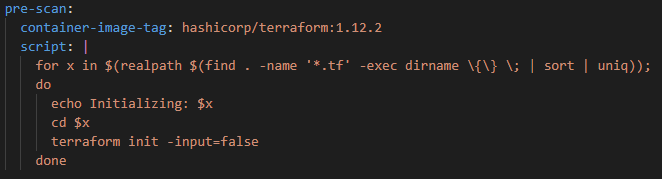
\includegraphics[scale=1]{graphics/scan-agent-pre-scan-script.png}
    \centering
    \caption{Scan Agent Pre-Scan Script Configuration YAML}
    \label{fig:pre-scan-script-config-yaml}
\end{figure}

When the container executes, the code from the repository is mapped to the \texttt{/code}
directory.  The environment variable \texttt{HOME} and the working directory are also set
to \texttt{/code}.  Changes to the content of the \texttt{/code} directory are persisted
after the container exits; all other changes made to the container file system are discarded
upon container exit.

The intention of this feature is to allow a small amount of preparation of the code
before it is sent to \cxone for scanning.  It is not intended as a full-featured code
build tool.  Any tooling configuration needed to support the pre-scan execution should be
included in the container image.  Scripts that require interactive input can not be supported.

The time taken to perform the pre-scan scripting for any script should generally be much
less than 10 minutes for any given code repository.  Pre-scan scripts that take a long time
run the risk of failing due to the message queue assuming that lack of acknowledgement
for the consumed scan delegation message means the agent is not working properly.  If
using RabbitMQ as the AMQP endpoint, it has a default server configuration \texttt{consumer-timeout}
set at 30 minutes (1800000ms).  This can be configured as a Policy via the RabbitMQ administrative
UI.  Figure \ref{fig:rmq-consumer-timeout} shows an example policy to increase the timeout to
3 hours.  It is applied on Queues with the name pattern \texttt{\^{}cx:res:Resolver Req.*} to limit
the change to queues used specifically by the Scan Agent.

\begin{figure}[h]
    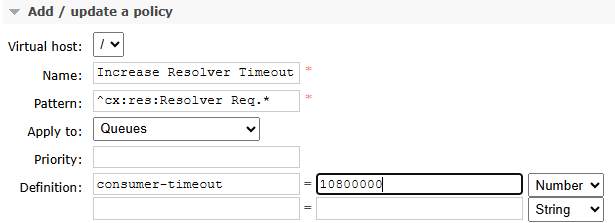
\includegraphics[scale=1]{graphics/scan-agent-consumer-timeout.png}
    \centering
    \caption{RabbitMQ Policy for Consumer Timeout}
    \label{fig:rmq-consumer-timeout}
\end{figure}


If the pre-scan script returns a non-zero exit status code,  the scan will have the resolver tag
\texttt{failure} but will still execute a scan.  Scripts should properly trap error conditions
to ensure successful execution.  For complex scripting needs, it is recommended that
the majority of the logic is built in to the container image with the pre-scan script only
serving to invoke the container's complex logic.


Container tags can reference publicly available images or private images.  The machine
where the Scan Agent is installed must have \texttt{docker} installed an configured
properly.  This includes performing a \texttt{docker login} as the \texttt{cx-scan-agent} user
account to properly cache any non-public container repository credentials.



\subsection{Security Considerations}\label{sec:scan-agent-security}

As briefly described in Section \ref{sec:scan-agent-security-considerations}, executing
part of a code build to extract a dependency tree or shell commands can pose some risks. For example,
tools like Gradle define the build definition in the programming language Groovy; this Groovy
code executes when Gradle loads the build definition.  Other tools even execute scripts defined
in the dependency package leading to the popular method of "typo-squatting" as a means to
perform a remote-code-execution (RCE) attack directly on unsuspecting developers.  Executing an
untrusted build definition or loading a dependency containing malware into a build system is
a risk that comes from using open-source software.

Since the risk of malicious builds is always possible, the deployment of the Scan Agent
can be configured to mitigate these risks.  The section for each platform's install makes specific
recommendations for a secure deployment of the Scan Agent.  The general recommendations
for all platform deployments are:

\begin{itemize}
  \item \textbf{Assume that anyone with administrative access to a server with a Scan Agent installed
    can intercept all secrets configured on the \cxoneflow server.}
  \item It is a best practice to not allow developers administrative control over the configuration and
    execution of the Scan Agent.
  \item Utilize file permissions on the secret values used by the agent to limit which running processes
    can read the contents of the secrets
  \item Use the recommended file system permissions for each platform's deployment.
  \item Find a logical grouping of agents for message queue credential assignment to better avoid
    impact if any credentials are misused.
  \item Use the message queue account security settings to limit message queue access to agents such that they are only
    able to receive and send events required for their specific operations.
  \item If the agent is invoking \scaresolver as a shell execution, utilize a "run-as" configuration to
    run the resolver as a low-privilege account.
  \item Utilize the \scaresolver docker execution capability to sandbox the dependency resolution in a container.
  \item Avoid configuring a Scan Agent instance to execute \scaresolver using both shell and container dependency resolution
    unless proper precautions have been taken to avoid privilege escalation exploits through the container file system overlay.
\end{itemize}


\subsubsection{Installing on Debian Linux}

The installation on Debian Linux platforms uses the Scan Agent Debian installer package
found with the \cxoneflow release.  The installer performs the following steps:

\begin{itemize}
  \item The agent is installed at the path \texttt{/opt/cxoneflow-scan-agent}
  \item The agent uses the configuration file \texttt{/etc/cxoneflow-scan-agent/config.yaml}
  \item A config template is installed at \texttt{/etc/cxoneflow-scan-agent/config.template.yaml}
  \item The agent is installed as a \texttt{systemd} service and registered to automatically run at system start.
  \item The non-login user \texttt{cx-scan-agent} is created and used to execute the \texttt{systemd} service.
  \item The non-login user \texttt{cx-scan-agent-rt} is created for use with the optional run-as isolation
    (see \intlink{par:shell-agent-isolation}{Shell Execution Isolation} for this optional configuration).
  \item A default directory for storing secrets is created at \texttt{/var/secrets} with permissions 500.
\end{itemize}

As part of the configuration, a work directory for the resolver will be required.  When this directory
is created, it is recommended to use the owner of \texttt{root:cx-scan-agent} and permissions of 770.  This
directory will primarily store temporary files used during the execution of \scaresolver.

The default secrets directory \texttt{/var/secrets} is created with ownership \texttt{cx-scan-agent:cx-scan-agent} and
permissions 500.  For secret files placed in this directory, it is recommended to each file is owned
by \texttt{cx-scan-agent:cx-scan-agent} with permissions of 400.  The permission of 400 will prevent 
build tools from reading the secrets when using the \intlink{par:shell-agent-isolation}{Shell Execution Isolation} option.

\paragraph{Controlling the Scan Agent}
\noindent\\The Scan Agent runs as a \texttt{systemd} service.  This allows the run status to be controlled
by commands such as "\texttt{systemctl start cxoneflow-scan-agent}" and\\"\texttt{systemctl stop cxoneflow-scan-agent}".

The Scan Agent runtime logs appear in \texttt{/var/log/syslog}.  To monitor the Scan Agent logs, execute the command
\\"\texttt{tail -f /var/log/syslog | grep scan.agent}".

Debug logging can be turned on for the Scan Agent by adding an environment variable in the \texttt{systemd}
service definition.  The following procedure will enable debug logging:

\begin{enumerate}
  \item Edit the file \texttt{/opt/cxoneflow-scan-agent/cxoneflow-scan-agent.service}
  \item Add the line "\texttt{Environment=LOG\_LEVEL=DEBUG}" under the existing line starting with\\\texttt{Environment}.
  \item Save the modifications to the \texttt{cxoneflow-scan-agent.service} file.
  \item Execute the command "\texttt{systemctl daemon-reload}".
  \item Execute the command "\texttt{systemctl restart cxoneflow-scan-agent}".
\end{enumerate}

\paragraph{Shell Execution}\label{par:agent-shell-execution}

\noindent\\Shell execution of \scaresolver is configured to use an instance of \scaresolver installed on the local system.
The execution of \scaresolverns, along with all build tools it invokes as part of the scan are executed with the \texttt{cx-scan-agent}
user.  The \texttt{cx-scan-agent} user is the executing user since the process is spawned from the \texttt{systemd} service that also
runs as the \texttt{cx-scan-agent} user.

The \texttt{cx-scan-agent} user is a non-login user that should have no access to do much other than run \texttt{git}, \scaresolverns, and
the build tools invoked as part of the dependency resolution.  The home directory for the \texttt{cx-scan-agent} user is dynamically set
to the value configured in \intlink{sec:scan-agent-work-path}{scan-agent-work-path} when \scaresolver is executed.  The location
of the home directory may have implications for how the build tools run.

Many build tools will have several places where they will look for configurations that are not explicitly placed in the build
definition.  In some cases, the configuration can exist in the home directory of the user running the build tool.  It may be necessary
to replicate build tool settings to the \intlink{sec:scan-agent-work-path}{scan-agent-work-path}.  If the build tools use a global location
for the settings, it may be necessary to adjust file/directory permissions to allow the \texttt{cx-scan-agent} user to access the global
configurations.

The build tools will often use the running user's home directory to write a package cache.  When the tool is invoked,
the running user's home directory is set to the value configured in \intlink{sec:scan-agent-work-path}{scan-agent-work-path}.
It may be possible to change the locations where the tools look for configuration or write package caches by configuring the
\intlink{sec:agent-resolver-opts}{resolver-opts} YAML element with
\extlink{https://docs.checkmarx.com/en/34965-132888-checkmarx-sca-resolver-configuration-arguments.html\#UUID-bc93274b-c1c7-ea47-9556-3bd8900711dc_id_CheckmarxSCAResolverConfigurationArguments-CustomParameters}
{custom parameters} passed to the build tools.

If transitioning to a configuration for \intlink{par:shell-agent-isolation}{Shell Execution Isolation}, the contents of the directory
defined in \intlink{sec:scan-agent-work-path}{scan-agent-work-path} will be owned by \texttt{cx-scan-agent:cx-scan-agent}.  This will likely
cause \scaresolver to fail since the change in configuration will cause the user running the tools to change to
\texttt{cx-scan-agent-rt}.  Most of the tools will require files and directories to be owned by\\\texttt{cx-scan-agent-rt:cx-scan-agent}.
It may be necessary to purge the \intlink{sec:scan-agent-work-path}{scan-agent-work-path} directory or selectively change
the ownership of build-tool related files/directories to \texttt{cx-scan-agent-rt:cx-scan-agent}.


\subparagraph{Shell Execution Isolation}\label{par:shell-agent-isolation}
\noindent\\Using the shell execution isolation configuration is an advanced option that requires granting limited sudoer privileges
to the \texttt{cx-scan-agent} user.  The sudoer privileges required are to allow the \texttt{cx-scan-agent} user to execute \scaresolver
as the user configured in \intlink{sec:agent-resolver-run-as}{resolver-run-as}.  The reason to use this option is to ensure that
the contents of the files located in the \intlink{sec:yaml-secret-root-path}{secret-root-path} can't be read while \scaresolver
is executing.\footnote{This assumes the recommendation of setting the permissions of each file in 
\intlink{sec:yaml-secret-root-path}{secret-root-path} to 400 has been followed.}

The installer creates a no-login user \texttt{cx-scan-agent-rt} as a default user that can be referenced in the \intlink{sec:agent-resolver-run-as}{resolver-run-as}
configuration.  Another user can be used provided the primary group membership is the \texttt{cx-scan-agent} group.  In most configurations, 
the \texttt{cx-scan-agent-rt} user will be sufficient.

The package installer does not configure this user with sudoer privileges by default primarily since the location of the \scaresolver
installation is unknown.  It is also best to allow a system administrator to be explicitly aware of users with sudoer privileges when installing
package.

To enable the \texttt{cx-scan-agent} user to have the required privileges, the following procedure can be followed:

\begin{enumerate}
  \item Execute the command "\texttt{visudo /etc/sudoers.d/00-cx-scan-agent}".
  \item Add the single line:\\"\texttt{cx-scan-agent ALL=(cx-scan-agent-rt) NOPASSWD: SETENV: /path/to/ScaResolver}"
  \item Save the \texttt{/etc/sudoers.d/00-cx-scan-agent} file.
  \item Configure the element \intlink{sec:agent-resolver-run-as}{resolver-run-as} in \texttt{/etc/cxoneflow-scan-agent/config.yaml} 
  with the user \texttt{cx-scan-agent-rt}.
  \item Restart the \texttt{systemd} service for the Scan Agent.
\end{enumerate}

Any configuration for tags that use shell execution of \scaresolver will now run as the user\\\texttt{cx-scan-agent-rt}.

\paragraph{Container Execution}
\noindent\\Container execution is supported using the \toolkit build environment that will extend a container image
specified in the \intlink{sec:agent-container-image-tag}{container-image-tag} YAML element.  The extended image
installs \scaresolver at the \texttt{systemd} service start.

The execution of \scaresolver is isolated from the underlying operating system by executing in the container image.
The container image, having all appropriate build tools and build tool configuration, will perform a dependency
tree resolution in the same way as it is done with shell execution.  This is similar to using
\intlink{par:shell-agent-isolation}{Shell Execution Isolation} by delegating execution to the docker image.

Assuming \texttt{docker} is installed, it is generally required to add the \texttt{cx-scan-agent} user to the \texttt{docker}
group using the command "\texttt{usermod -a -G docker cx-scan-agent}".  This allows the \texttt{cx-scan-agent} user to execute
commands to build and run containers.

\subparagraph{Container Execution Security}
\noindent\\The installation of \texttt{docker} is usually done such that the \texttt{docker} daemon runs with
root privileges.  For Scan Agent configurations that allow 
\intlink{par:agent-shell-execution}{Shell Execution} along with container execution, this capability could pose
the risk of privilege escalation via the \texttt{docker} runtime.

If not configured for \intlink{par:shell-agent-isolation}{Shell Execution Isolation}, it is possible that
executing build tools via \scaresolver running as the \texttt{cx-scan-agent} user can escalate privileges
to read and write files with root privileges.  This is due to the \texttt{cx-scan-agent} user being a member of
the \texttt{docker} group and \scaresolver executing as \texttt{cx-scan-agent}.  


\subsection{Scan Agent YAML Configuration}\label{sec:agent-yaml-config}

The Scan Agent's YAML configuration is deployed after the agent is installed.
Many of the elements share format with the \intlink{sec:yaml-config}{server's configuration elements}. 


Figure \ref{fig:scan-agent-config-yaml} shows an example of the serviced tag configurations for 
a Scan Agent YAML configuration.  The example YAML can be downloaded from the \cxoneflow YAML
example release artifacts.

\begin{figure}[h]
    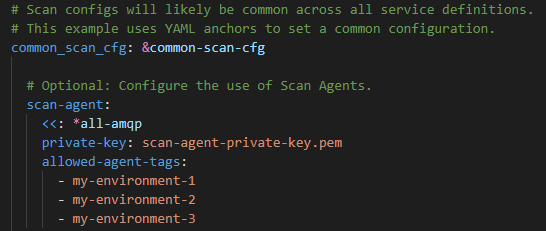
\includegraphics[scale=1]{graphics/scan-agent-config-yaml.png}
    \centering
    \caption{Scan Agent Configuration YAML}
    \label{fig:resolver-agent-config-yaml}
\end{figure}

\pagebreak

\subsubsection{Scan Agent YAML Configuration Tree}\label{sec:agent-yaml-root}

\dirtree{%
    .1 <root>.
    .2 \intlink{sec:yaml-secret-root-path}{secret-root-path}\DTcomment{[Required]}.
    .2 \intlink{sec:agent-serviced-tags}{serviced-tags}\DTcomment{[Required]}.
    .3 \intlink{sec:agent-tag}{<agent tag>}\DTcomment{[At least 1 required]}.
    .4 \intlink{sec:yaml-generic-amqp}{amqp}\DTcomment{[Optional] Default: localhost}.
    .5 \intlink{sec:yaml-generic-amqp-amqp-password}{amqp-password}\DTcomment{[Optional]}.
    .5 \intlink{sec:yaml-generic-amqp-amqp-url}{amqp-url}\DTcomment{[Required]}.
    .5 \intlink{sec:yaml-generic-amqp-amqp-user}{amqp-user}\DTcomment{[Optional]}.
    .5 \intlink{sec:yaml-generic-ssl-verify}{ssl-verify}\DTcomment{[Optional] Default: True}.
    .4 \intlink{sec:agent-disable-resolver}{disable-resolver}\DTcomment{[Optional] Default: False}.
    .4 \intlink{sec:agent-pre-scan}{pre-scan}\DTcomment{[Optional]}.
    .5 \intlink{sec:agent-pre-scan-container-image-tag}{container-image-tag}\DTcomment{[Required]}.
    .5 \intlink{sec:agent-pre-scan-resolver-before-script}{resolver-before-script}\DTcomment{[Optional] Default: False}.
    .5 \intlink{sec:agent-pre-scan-run-as-agent}{run-as-agent}\DTcomment{[Optional] Default: True}.
    .5 \intlink{sec:agent-pre-scan-script}{script}\DTcomment{[Required]}.
    .5 \intlink{sec:agent-pre-scan-shell}{shell}\DTcomment{[Optional] Default: /bin/sh}.
    .4 \intlink{sec:agent-public-key}{public-key}\DTcomment{[Required]}.
    .4 \intlink{sec:agent-resolver-opts}{resolver-opts}\DTcomment{[Optional] Default: None}.
    .4 \intlink{sec:agent-resolver-path}{resolver-path}\DTcomment{[Required if not \texttt{run-with-container}]}.
    .4 \intlink{sec:agent-resolver-run-as}{resolver-run-as}\DTcomment{[Optional] Default: run as service user}.
    .4 \intlink{sec:scan-agent-work-path}{scan-agent-work-path}\DTcomment{[Optional] Default: /tmp}.
    .4 \intlink{sec:agent-run-with-container}{run-with-container}\DTcomment{[Required if not \texttt{resolver-path}]}.
    .5 \intlink{sec:agent-container-image-tag}{container-image-tag}\DTcomment{[Required]}.
    .5 \intlink{sec:agent-supply-chain-toolkit-path}{supply-chain-toolkit-path}\DTcomment{[Required]}.
    .5 \intlink{sec:agent-use-running}{use-running-gid}\DTcomment{[Optional] Default: True}.
    .5 \intlink{sec:agent-use-running}{use-running-uid}\DTcomment{[Optional] Default: True}.
}

\input{resolver/yaml/root.tex}
\input{resolver/yaml/serviced-tags.tex}
\subsubsection{<agent tag>.disable-resolver}\label{sec:agent-disable-resolver}
Defaults to \texttt{False}.  Set to \texttt{True} to disable execution of \scaresolver.  This is typically used with 
\intlink{sec:agent-pre-scan}{pre-scan} configured to execute a scan step that does not require the use of \scaresolver.

If this is set to \texttt{True}, options \intlink{sec:agent-resolver-path}{resolver-path} and 
\intlink{sec:agent-run-with-container}{run-with-container} are ignored.


\subsubsection{<agent tag>.pre-scan}\label{sec:agent-pre-scan}
This element contains elements to support \intlink{sec:scan-agent-prescan}{pre-scan scripting}.

\subsubsection{<agent tag>.pre-scan.container-image-tag}\label{sec:agent-pre-scan-container-image-tag}
This is a tag to a container image where the configured \intlink{sec:scan-agent-prescan}{script} will execute.

\subsubsection{<agent tag>.pre-scan.resolver-before-script}\label{sec:agent-pre-scan-resolver-before-script}
If set to \texttt{False} (the default), \scaresolver executes after the \intlink{sec:agent-pre-scan-script}{pre-scan script}.
If set to \texttt{True}, \scaresolver executes before the \intlink{sec:agent-pre-scan-script}{pre-scan script}. If \scaresolver
execution has been disabled with the \intlink{sec:agent-disable-resolver}{disable-resolver} option, this setting is ignored.


\subsubsection{<agent tag>.pre-scan.run-as-agent}\label{sec:agent-pre-scan-run-as-agent}
The default setting is \texttt{True}.  If set to \texttt{True}, the container runs with the UID:GID of
the scan agent.  This is to allow for the overlay file system to read/write to the mapped code directory
while executing the pre-scan script.  If set to \texttt{False}, the container runs as the container default
user.

When running as the container default user, anything written to the mapped code directory may prevent the scan
agent from having read/write access after the container exits.  The pre-scan script should set the read/write
permissions on or remove files written during the container execution prior to exiting the container.  This will
allow the scan agent to remove the temporary copy of the code when the pre-scan execution is complete.


\subsubsection{<agent tag>.pre-scan.script}\label{sec:agent-pre-scan-script}
The script to execute in the running container image.  This can be a single line or a multi-line
string using the \extlink{https://yaml.org/spec/1.2.2/\#812-literal-style}{YAML literal scalar style} syntax
by using the bar character ("\texttt{|}") as the value and indenting the next several lines to form the
complete script.


\subsubsection{<agent tag>.pre-scan.shell}\label{sec:agent-pre-scan-shell}
By default, the pre-scan script will execute in the container's shell located at \texttt{/bin/sh}.  This is a standard shell location
in most Linux distributions.  The path to an alternate shell on the container image can optionally be defined here.

\subsubsection{<agent tag>.public-key}\label{sec:agent-public-key}
The value specifies a file name found under the path defined by \texttt{secret-root-path} containing a 
public key that matches the server's configured \intlink{sec:yaml-resolver-private-key}{\texttt{private-key}} setting.


\subsubsection{<agent tag>.resolver-opts}\label{sec:agent-resolver-opts}
This is a dictionary of
\extlink{https://docs.checkmarx.com/en/34965-132888-checkmarx-sca-resolver-configuration-arguments.html\#UUID-bc93274b-c1c7-ea47-9556-3bd8900711dc_id_CheckmarxSCAResolverConfigurationArguments-ConfigurationArguments-TablesandSamples}{configuration arguments}
passed to \scaresolver when executing.  The options are used to provide static values for resolver execution configuration.  Some of the
options may clash with execution options provided by the agent; options that would clash with how the agent executes \scaresolver are ignored.  

The \texttt{resolver-opts} section is a dictionary of key and key/value pairs that correspond to
\extlink{https://docs.checkmarx.com/en/34965-132888-checkmarx-sca-resolver-configuration-arguments.html}{command line options} for \scaresolver.
The options that can be used are limited considering some of the options are used by the \cxoneflow integration to execute \scaresolver.

These options, if set, will be ignored:

\begin{itemize}
  \item logs-path
  \item a | account
  \item containers-result-path
  \item resolver-result-path
  \item project-name
  \item authentication-server-url
  \item p | password
  \item sso-provider
  \item sca-app-url
  \item s | scan-path
  \item server-url
  \item u | username
  \item project-tags
  \item scan-tags
  \item bypass-exitcode
  \item no-upload-manifest
  \item help
  \item manifests-path
  \item t | project-teams
  \item q | quiet
  \item save-evidence-path
  \item severity-threshold
  \item report-content
  \item report-extension
  \item report-path
  \item report-type
  \item sast-result-path
  \item cxpassword
  \item cxuser
  \item cxprojectid
  \item cxprojectname
  \item cxserver
\end{itemize}

\subsubsection{<agent tag>.resolver-path}\label{sec:agent-resolver-path}
The path to the \scaresolver executable that has been installed on the system running the Scan Agent.


\subsubsection{<agent tag>.resolver-run-as}\label{sec:agent-resolver-run-as}
The name of a user account that will run the \scaresolver when executed in a shell (but not as a container).  This
is an advanced configuration that will require additional configuration for your platform.  

If not provided, the \scaresolver is executed as the same user that is running the Scan Agent service.

\subsubsection{<agent tag>.scan-agent-work-path}\label{sec:scan-agent-work-path}
A path where temporary files are written during the operation of the Scan Agent.  This also serves as the home
directory for the Scan Agent user and the user defined in \texttt{resolver-run-as}.

\subsubsection{<agent tag>.run-with-container}\label{sec:agent-run-with-container}
A YAML dictionary with key/value pairs used to define running \scaresolver in a container.  If this is supplied,
the configured \texttt{resolver-path} is ignored and \scaresolver will not be invoked in a shell.  The dependency
tree collected by \scaresolver will be done by executing build tools defined in the container.  This is useful for
organizations that utilize containerized build environments in their CI/CD pipeline build scripts.

The use of containers to run \scaresolver is not supported on Windows platforms.

\subsubsection{<agent tag>.run-with-container.container-image-tag}\label{sec:agent-container-image-tag}
The container tag that is found in one of the logged-in container registries.  This container tag is used by the \toolkit
to create an extended image with \scaresolver installed.

\subsubsection{<agent tag>.run-with-container.supply-chain-toolkit-path}\label{sec:agent-supply-chain-toolkit-path}
The path where the \toolkit build environment is installed.

\subsubsection{<agent tag>.run-with-container.use-running-gid and\\<agent tag>.run-with-container.use-running-uid}\label{sec:agent-use-running}
These options are True by default.  This causes the image built by the \toolkit to use the
UID and primary GID of the user running the Scan Agent when defining a non-root
user in the extended image.  

The reason for this is that when \scaresolver is executed in the container, temporary paths
in the \texttt{resolver-work-path} are mapped to the container.  Files created by the container
will have the UID/GID of the running container's user when created.  Since the UID/GID of the
container matches the UID/GID of the Scan Agent, the files that remain after
the container exits can be controlled by the Scan Agent.

Setting these values to False should only be done in circumstances where the UID/GID for written files
should be defined by the container.  This scenario may never practically exist.



\subsection{Resolver Configuration Recommendations}

The YAML configuration option \intlink{sec:agent-resolver-opts}{resolver-opts} can be used to provide
configuration options for \scaresolver during execution.  This section discusses recommended
configuration options.

\subsubsection{break-on-manifest-failure}\label{sec:break-manifest}

This is a boolean option that is passed to \scaresolver as the argument \texttt{--break-on-manifest-failure}.  It is recommended
that this is set in the \intlink{sec:agent-resolver-opts}{resolver-opts} configuration.  This will cause any manifest failures
encountered when running \scaresolver to flag the scan with the resolver tag of \textbf{failed}.  If this option is not included,
all scans will have a resolver tag of \textbf{success} regardless of if resolution of any dependency trees failed when
executing \scaresolverns.

The reason \scaresolver should be configured to run with this option is to make it easy to filter a list of scans by resolver
failure status.  All SCA scans are reported as successfully completed if the dependency tree resolution executes to
any type of completion.  The dependency resolution may completely or partially fail but the scan status will reflect
as a successful scan.  Any partial results will be reported but it requires some manual review of logs to understand if there
were any partial dependency tree resolution failures.

\subsubsection{scan-containers}
This is a boolean option that is passed to \scaresolver as the argument \texttt{--scan-containers}.  It is recommended that
this option is \textbf{not} set in the \intlink{sec:agent-resolver-opts}{resolver-opts} configuration.

There are a few reasons for omitting this flag; the main reason is that container security scans have moved away from
using \scaresolver to perform the scan.  Container security scans are now an independent scan option and no longer
report results provided by \scaresolver when used by \cxonens.  This option may remain in \scaresolver for backwards
compatibility with other Checkmarx products.

\subsection{Limitations}
Please note the following limitations apply when using the Scan Agent:

\begin{itemize}
  \item Server-side configurations with \texttt{clone-auth} using SSH keys will fail.
  \item Windows base container images can not be used to run \scaresolver in a container.  Only Linux base images are supported.
  \item The Container Security scans recently moved away from using \scaresolverns, thus container scans will currently
    execute in the \cxoneflow server side environment.
\end{itemize}

